%\documentclass[twocolumn]{article}
%\usepackage{graphicx}

%\begin{document}

\subsubsection{Laser Spectroscopy in
Energy and Time Domain} \index{Materny, Arnulf}

\paragraph{Research Team}
Dr.\ Dr.\ Arnulf Materny (Professor), Dr.\ Thorsten Balster (Research Associate), Patrice Donfack (PhD Student), Rasha Hassanin (PhD Student), Jakow Konradi (PhD Student), Vinu Namboodiri (PhD Student), Malte Sackmann (PhD Student), Abraham Scaria (PhD Student), Safieh Tork (PhD Student), Sidhant Bom (Master Student), Khadga Karki (Master Student)\\

Laser spectroscopy in the energy and time domain is applied to
investigate and control the structure and dynamics of molecules. Raman scattering is used as optical tool for the identification of carcinogenic tissue and marker substances (coop.\ Brix and Lerchl, IUB; Wenk, Klinikum Bremen-Nord; Hu, China) as well as for the characterization of food. For this, techniques are developed, which are based on the surface enhancement of the Raman signal (SERS) by nanostructured metal surfaces (coop.\ Wagner, IUB) and nano metal clusters. Using femtosecond time-resolved laser spectroscopy, the ultrafast energy transport in molecules is investigated and controlled. Examples are the internal conversion processes and the inter-molecular energy flow for pigment molecules relevant to photosynthesis. In order to realize ``artificial photosystems'', the molecules are embedded in nanometer-sized silica cages (coop.\ Richards, IUB). The control of vibrational dynamics, which is relevant for selective chemistry, is achieved by shaping the femtosecond laser pulses in a self-learning loop approach (coop.\ Kleinekath\"{o}fer, IUB).



\paragraph{Highlights}

Our research in 2006 concentrated mainly on three fields.

\textit{Surface Enhanced Raman Scattering (SERS) for Cancer
Diagnosis and Food Characterization} --- In the Raman laboratory,
we make use of the fact that the inelastic light scattering
process can be enhanced considerably if the investigated molecules
are adsorbed on the surfaces of nanometer-sized metal structures.
In a cooperation with Prof.\ Wagner, arrays of gold nanostructures
were produced in a well-defined way by means of electron
lithography. Their usability for SERS was investigated in detail.
The SERS technique enabled us to obtain spectra of human tissue,
which we have investigated to establish a fast method for
non-invasive cancer diagnosis together with our Chinese partners
from Wuhan University (Prof.\ Hu). Together with Prof.\ Brix, we
also did experiments on \textit{e.g.} cysteine proteinase
cathepsin B, which is a possible cancer marker. A new
collaboration with Prof.\ Lerchl was initiated, where animal
tissue will be investigated. Human carcinogenic samples will be
provided by the Klinikum Bremen-Nord (Prof. Wenk). First
experiments on coffee, where standard Raman spectroscopy is not
successful resulted in SERS spectra, which appear to be
characteristic for the used coffee samples. To further follow this
interesting application in food chemistry, a new Ph.D.\ student
started her work focussing on this theme.

\textit{Control of Vibrational Dynamics on a Femtosecond
Time-Scale} --- In the femtosecond laser laboratory, we have
continued our project on femtosecond control of molecular
vibration modes by means of four-wave mixing (FWM). Here, two
laser pulses excite the molecular vibrations in phase and a
time-delayed third laser pulse probes the resulting mode
distribution. A selective excitation of a vibrational motion in
molecules is decisive for the well-defined driving of chemical
reactions. By shaping the femtosecond laser pulses, we were able
to enhance and/or suppress vibrational modes. The goal was
achieved by using an evolutionary algorithm controlling the pulse
shaper in a closed loop, where the nonlinear Raman scattering
signal served as fitness function for the optimization. For the
theoretical description of the dynamics the collaboration with
Prof.\ Kleinekath\"{o}fer was continued.

\begin{figure}[ht]
  \begin{center}
    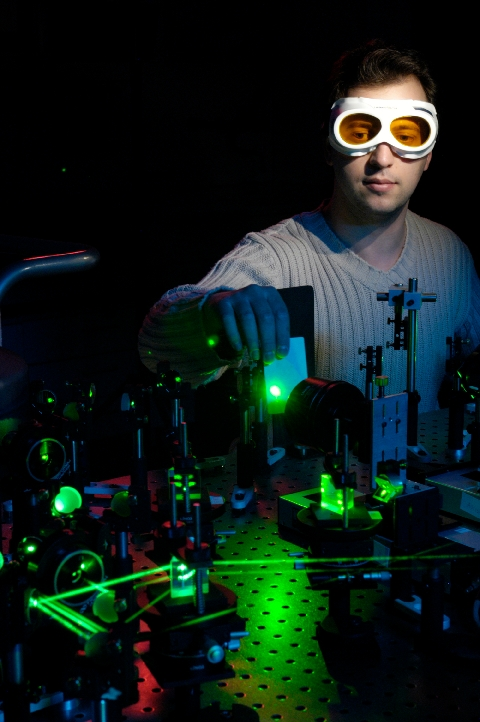
\includegraphics[width=6cm]{Materny/materny_2006_fig.jpg}
    \mycaption{Part of the optical setup used for femtosecond time-resolved four-wave mixing spectroscopy.}\label{fig:materny}
   \end{center}
\end{figure}

\textit{Energy Transfer Dynamics in Artificial Light Harvesting
Systems} --- In a collaboration with Prof.\ Richards, pigment
molecules, which are part of the natural photosystem, were
enclosed into porous silica cages of few nanometers in diameter.
The goal is to mimic natural light harvesting in artificial
matrices and to finally convert light energy into chemical energy.
The ultrafast intra- and intermolecular energy transfer steps of
these pigment molecules were studied by means of femtosecond
time-resolved transient absorption or diffuse reflection
experiments. Very recently, we succeeded in observing for the
first time the changed behavior due to the nanocage environment.


\paragraph{Organization}

\begin{enumerate}
\item European Conference on Nonlinear Optical Spectroscopy, Bratislava, Slovakia
\item Symposium on Femtosecond Time-Resolved Spectroscopy, Sun Yat-sen University, Guangzhou City, China (together with Dr.\ Chen Jian)
\end{enumerate}

\paragraph{Collaborations}
\begin{enumerate}
\item {\sl International University Bremen}\\
      Prof.\ Veit Wagner\\
      Nanostructered Surfaces as Substrates for Surface-Enhanced Raman Spectroscopy (SERS)
\\
      Prof.\ Ryan M.\ Richards\\
      Synthesis of Artificial Environments for Pigment Molecules (Artificial Photosystem)
\\
      Prof.\ Klaudia Brix\\
      Cancer biomarkers and cancerogenic cells for SERS investigation.
\\
      Prof.\ Alexander Lerchl\\
      Cancerogenic animal tissue for SERS investigation.
\item {\sl University of Chemnitz / International University Bremen}\\
      Prof.\ Ulrich Kleinekath\"{o}fer\\
      Theoretical Models for Quantum Control of Chemical Reactions.
\item {\sl University of W\"{u}rzburg}\\
      Prof.\ Volker Engel\\
      Simulation of Molecular Dynamics.
\item {\sl Klinikum Bremen-Nord}\\
      Prof.\ Heiner H.\ Wenk\\
      Cancerogenic human tissue for SERS investigation.
\item {\sl Wuhan University, Wuhan, China}\\
      Prof.\ Jiming Hu\\
      Development and Application of New Raman Techniques for Cancer Diagnosis.
\item {\sl Banaras Hindu University, Varanasi, India}\\
      Prof.\ Birendra P.\ Asthana\\
      Raman Spectroscopy for the Investigation of Host-Guest Interactions.
\end{enumerate}


\paragraph{Grants}

\begin{enumerate}
\item Funded by DFG, \emph{Frequenzaufgel\"{o}ste nichtlineare Spektroskopie mit spektral breiten Femtosekundenpulsen
durch die Anwendung optimaler Kontrollschemata}, Project MA
1564/10-1,2 (December 2003 - July 2007)

\item Funded by DFG, \emph{Frequenzaufgel\"{o}ste nichtlineare Spektroskopie mit spektral breiten
Femtosekundenpulsen durch die Anwendung optimaler Kontrollschemata},
Project MA 1564/10-1,2 (November 2004 - December 2007).

\item Funded by DAAD-PPP, \emph{Development and Application of New Raman Techniques for Cancer Diagnosis'',
DAAD/China Scholarship Council Grant} ,  D/05/06942  (January 2006 -
December 2007)
\end{enumerate}


\paragraph{Other Support Grants}

\begin{enumerate}

\item Alexander-von-Humboldt Foundation, ``Electric Field Effects of the Ultrafast Dynamics in Molecular Systems'',
Humboldt Fellowship (Dr.\ Ajay Singh) (2005--2006).


\item DAAD, ``Raman Spectroscopy on Animal and Human Tissue'',  Ph.D.\ Fellowship (Patrice Donfack, Cameroon) (2005--2009).

\item DFG, ``SERS for Cancer Diagnosis'', Guest Professorship (Prof.\ Jiming Hu, China) (2006).

\item Slovensk\'{a} akademick\'{a} informa\v{c}n\'{a} agent\'{u}ra (SAIA), ``Controlling the Elementary Steps of Chemical Reaction by Femtosecond Pulse Shaping'', Fellowship (Attila Gaal, Slovakia) (2006).

\item Ministry of Higher Education of Egypt, ''Raman Techniques for the Characterization of Food'', Ph.D. Fellowship (Rasha Hassanin, Egypt) (2006--2009).
\end{enumerate}

\paragraph{Awards, Prizes}

\begin{enumerate}
\item Member of Engineering \& Physical Sciences Research Council (EPSRC) College, U.K.
\item Fellow of the World Innovation Foundation (WIF)
\item Bunsen-Dozent for the Bunsen-Gesellschaft (Physical Chemistry) at the IUB
\item Editorial Board Member of the Asian Chemistry Letters
\item Guest Professorship at Wuhan University, China (2006--2008)
\end{enumerate}

\nocite{KON-7-06, KON-697-06, KON-289-06, SAC-305-06, MAT-226-06, SAC-online-06, SCA-press-06, KON-press-06}

%\bibliography{Materny_2006}
%\bibliographystyle{unsrt}

%\end{document}
